%=====================================================================
\section{Counterfactual Fusion Design and the Rule--Outcome Frontier}\label{sec:counterfactual}
%=====================================================================

The problem asks not only to estimate the hidden vote but to advise the producers on the
fusion rule. To move from a handful of named controversies to a systematic comparison, we
replay three decades of eliminations under a continuous family of rules and measure how often
each rule reproduces the observed outcome. This section states the replay design, reports the
resulting frontier, and --- importantly --- delimits what the exercise can and cannot prove.

\subsection{Replay Design}\label{sec:replaydesign}

For a fixed weight $w\in[0,1]$ we form the counterfactual combined score

\begin{equation}
\label{eq:weightedscore}
  C_{i,sw}(w) \;=\; w\,q^J_{i,sw} \;+\; (1-w)\,\tilde q^F_{i,sw},
  \qquad i\in S_{sw},
\end{equation}

and predict that the couple minimising $C_{i,sw}(w)$ is eliminated. The endpoints are
informative: $w=1$ is a judge-only rule using official scores exclusively, while $w=0$ is a
fan-only rule. The historical percent rule corresponds to $w=0.5$ up to the renorm\-alisation
used here. An ordinal analogue replaces both shares by their within-week ranks,

\begin{equation}
\label{eq:weightedrank}
  C^{\rm rank}_{i,sw}(w) \;=\; w\,r^J_{i,sw} \;+\; (1-w)\,r^F_{i,sw},
\end{equation}

with the couple \emph{maximising} $C^{\rm rank}$ eliminated, since rank $1$ denotes the best
couple. We scan $w$ on a grid of $21$ points and compute, for each, the fraction of the $266$
eliminating weeks in which the predicted and observed eliminations coincide. All shares are
within-week renormalised so that the two channels enter on the same scale
(Section~\ref{sec:eda_source}).

\paragraph{A necessary caveat on circularity.} The reconstructed fan share is drawn from a
polytope whose inequalities \emph{enforce the observed elimination}. Consequently, for any
$w$ that gives the fan channel appreciable weight, a high consistency rate is a designed
property of the reconstruction, not out-of-sample predictive accuracy. We therefore shade the
region $w\lesssim0.55$ in Figure~\ref{fig:frontier} and refrain from interpreting it as model
validation. Exactly one point on the curve is free of this circularity: at $w=1$ the score
contains no reconstructed quantity at all, and the resulting $0.444$ is the judge-only
benchmark of Section~\ref{sec:judgebaseline}. The legitimate reading of the frontier is thus
about \emph{sensitivity} --- how quickly consistency degrades as the audience channel is
removed --- not about forecast skill. A genuine out-of-sample test would require the Model~2
generative likelihood discussed in Section~\ref{sec:m2_status}.

\begin{figure}[H]
\centering
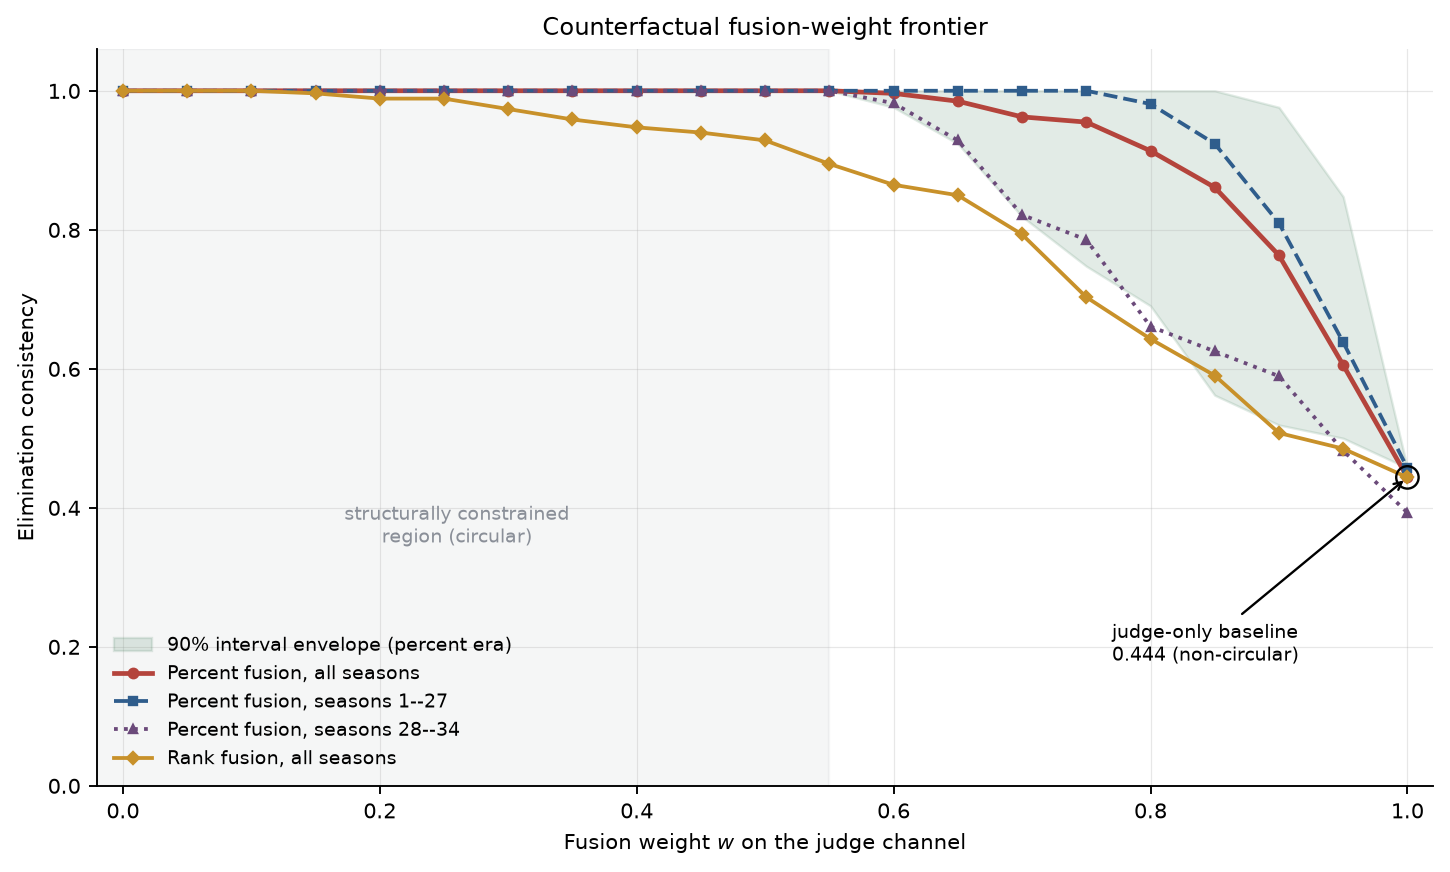
\includegraphics[width=0.88\textwidth]{figures_ext/fig07_fusion_weight_frontier.png}
\caption{Counterfactual fusion-weight frontier. Elimination consistency as the weight $w$ on
the judge channel varies from $0$ (fan-only) to $1$ (judge-only). The shaded left region is
structurally constrained and must not be read as predictive accuracy. The green envelope shows
the range obtained by replacing the posterior median with the $5\%$ and $95\%$ fan-share bounds.
The circled point is the non-circular judge-only baseline.}
\label{fig:frontier}
\end{figure}

\subsection{The Frontier and What It Shows}

Table~\ref{tab:weights} reports the full grid. Three features stand out.

\emph{(i) The judge channel alone is insufficient.} At $w=1$ consistency is $0.444$ pooled,
$0.457$ in seasons 1--27 and $0.393$ in seasons 28--34. No amount of reweighting can make a
judge-only rule reproduce more than about half of the observed eliminations. This is the
model-free anchor of the whole analysis.

\emph{(ii) Consistency degrades smoothly, not abruptly, and later seasons degrade faster.} At
$w=0.75$ the pooled rate is $0.955$, but the percent era remains at $1.000$ while the
bottom-two era has already fallen to $0.786$; at $w=0.8$ the split widens to $0.981$ versus
$0.661$. The late seasons are more sensitive to the removal of audience weight because the
judge save introduces a second, judge-driven decision that the combined score cannot express.
This is a quantitative complement to the $0.400$ hit-rate finding.

\emph{(iii) Rank fusion is more weight-sensitive than percent fusion.} The ordinal curve falls
to $0.929$ at $w=0.5$, $0.865$ at $w=0.6$, $0.703$ at $w=0.75$ and $0.508$ at $w=0.9$,
whereas the percent curve stays above $0.96$ until $w=0.7$. Ordinal ranks are coarse (only
$n_{sw}$ distinct values) and ties are frequent, so small changes in $w$ can reorder two
near-equal couples. This is the same mechanism that makes rank fusion favour fan favourites:
it discards the magnitude of a judge advantage that percent fusion would preserve.

% AUTO-GENERATED table — values computed by analyze_extended.py
\begin{table}[H]
\centering
\caption{Counterfactual elimination consistency as the fusion weight $w$ on the judge channel varies. Score $=w\,q^J+(1-w)\,\hat q^F$; the predicted elimination is the couple minimising the score. Percent-era = seasons 1--27, bottom-two era = seasons 28--34. The rank column uses $w\,r^J+(1-w)\,r^F$ on ordinal ranks.}
\label{tab:weights}
\begin{tabular}{lcccc}
\toprule
$w$ (judge weight) & All seasons & Percent era & Bottom-two era & Rank fusion \\ 
\midrule
0.0 & 1.000 & 1.000 & 1.000 & 1.000 \\ 
0.1 & 1.000 & 1.000 & 1.000 & 1.000 \\ 
0.2 & 1.000 & 1.000 & 1.000 & 0.989 \\ 
0.3 & 1.000 & 1.000 & 1.000 & 0.974 \\ 
0.4 & 1.000 & 1.000 & 1.000 & 0.947 \\ 
0.5 & 1.000 & 1.000 & 1.000 & 0.929 \\ 
0.6 & 0.996 & 1.000 & 0.982 & 0.865 \\ 
0.7 & 0.962 & 1.000 & 0.821 & 0.793 \\ 
0.8 & 0.913 & 0.981 & 0.661 & 0.643 \\ 
0.9 & 0.763 & 0.809 & 0.589 & 0.507 \\ 
1.0 & 0.444 & 0.457 & 0.393 & 0.444 \\ 
\bottomrule
\end{tabular}
\end{table}


\subsection{Uncertainty-Aware Replay}\label{sec:intervalreplay}

Because the posterior median is only one point in a wide feasible set, a replay that uses it
alone overstates what is identified. We therefore repeat the percent-era scan three times,
substituting the $5\%$ lower bound $\hat q^F_{5}$, the median, and the $95\%$ upper bound
$\hat q^F_{95}$ for the fan channel. Figure~\ref{fig:intervalreplay} shows the resulting
envelope. For $w\le0.5$ all three curves agree at $1.000$, so conclusions in the
historically relevant range are interval-robust. At $w=0.75$ the lower-bound replay falls to
$0.748$ while the upper bound stays at $1.000$; at $w=0.9$ the spread is $0.519$ to $0.976$.
Any claim about high-weight rules is therefore sensitive to where in the credible set the true
vote lies, and should be reported with this envelope rather than as a single number.

\begin{figure}[H]
\centering
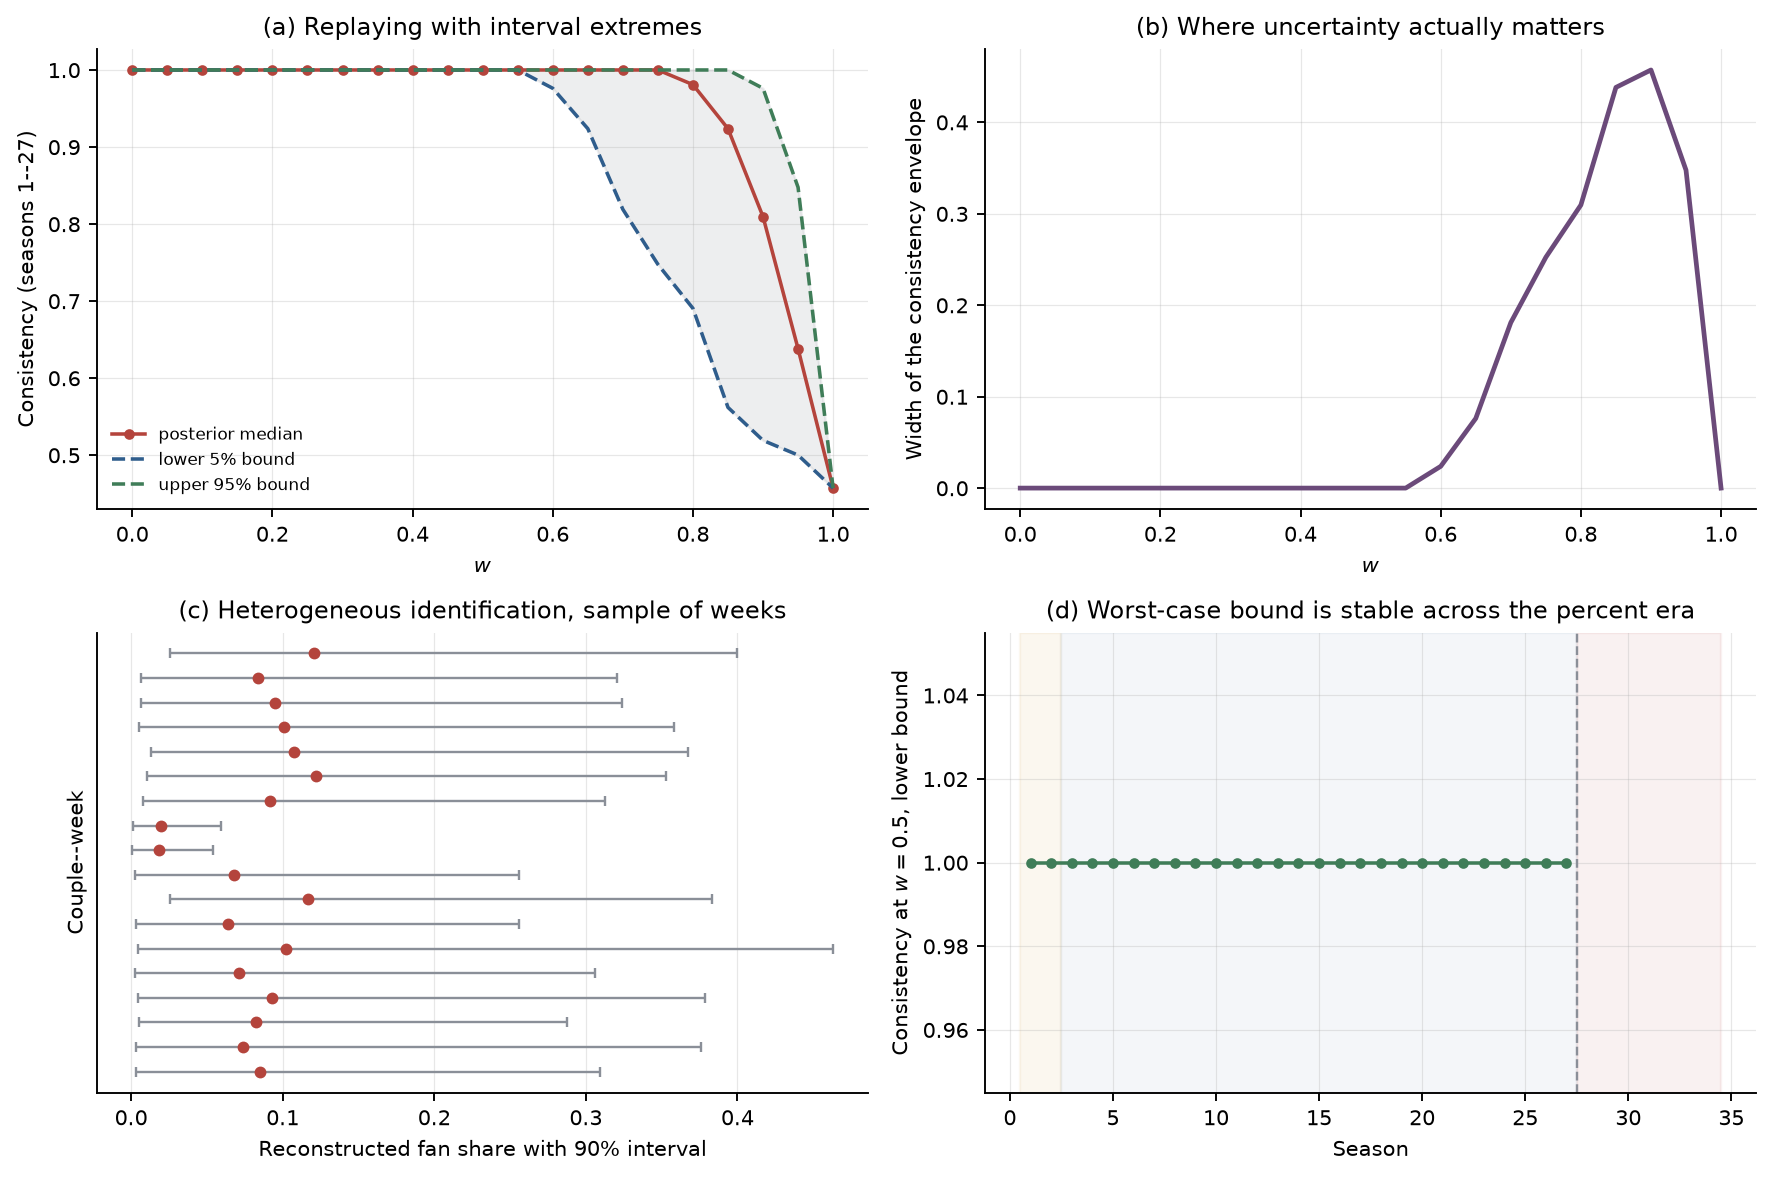
\includegraphics[width=0.94\textwidth]{figures_ext/fig13_interval_robust_replay.png}
\caption{Uncertainty-aware counterfactual replay. (a) Consistency under the median, $5\%$ and
$95\%$ fan-share surfaces for seasons 1--27. (b) Width of the envelope as a function of $w$.
(c) A sample of individual $90\%$ intervals illustrating heterogeneous identification.
(d) Worst-case consistency at $w=0.5$ by season, which is stable across the percent era.}
\label{fig:intervalreplay}
\end{figure}

\subsection{How Often Do the Two Historical Rules Disagree?}

A separate, non-circular question is whether the rank and percent rules would have eliminated
\emph{different} couples. Using the materialised percent-combined and rank-combined columns,
we compare the two predicted eliminations week by week. They disagree in \textbf{24 of 266}
eliminating weeks, i.e.\ $\mathbf{9.02\%}$ of the time. Split by regime, the disagreement rate
is $0.0\%$ in the two rank-era seasons, $9.41\%$ in the percent era and $13.55\%$ in the
bottom-two era. Figure~\ref{fig:disagreement} maps where those weeks occur: they are scattered
rather than concentrated in a single season, but cluster in weeks with large fields and close
combined scores.

\begin{figure}[H]
\centering
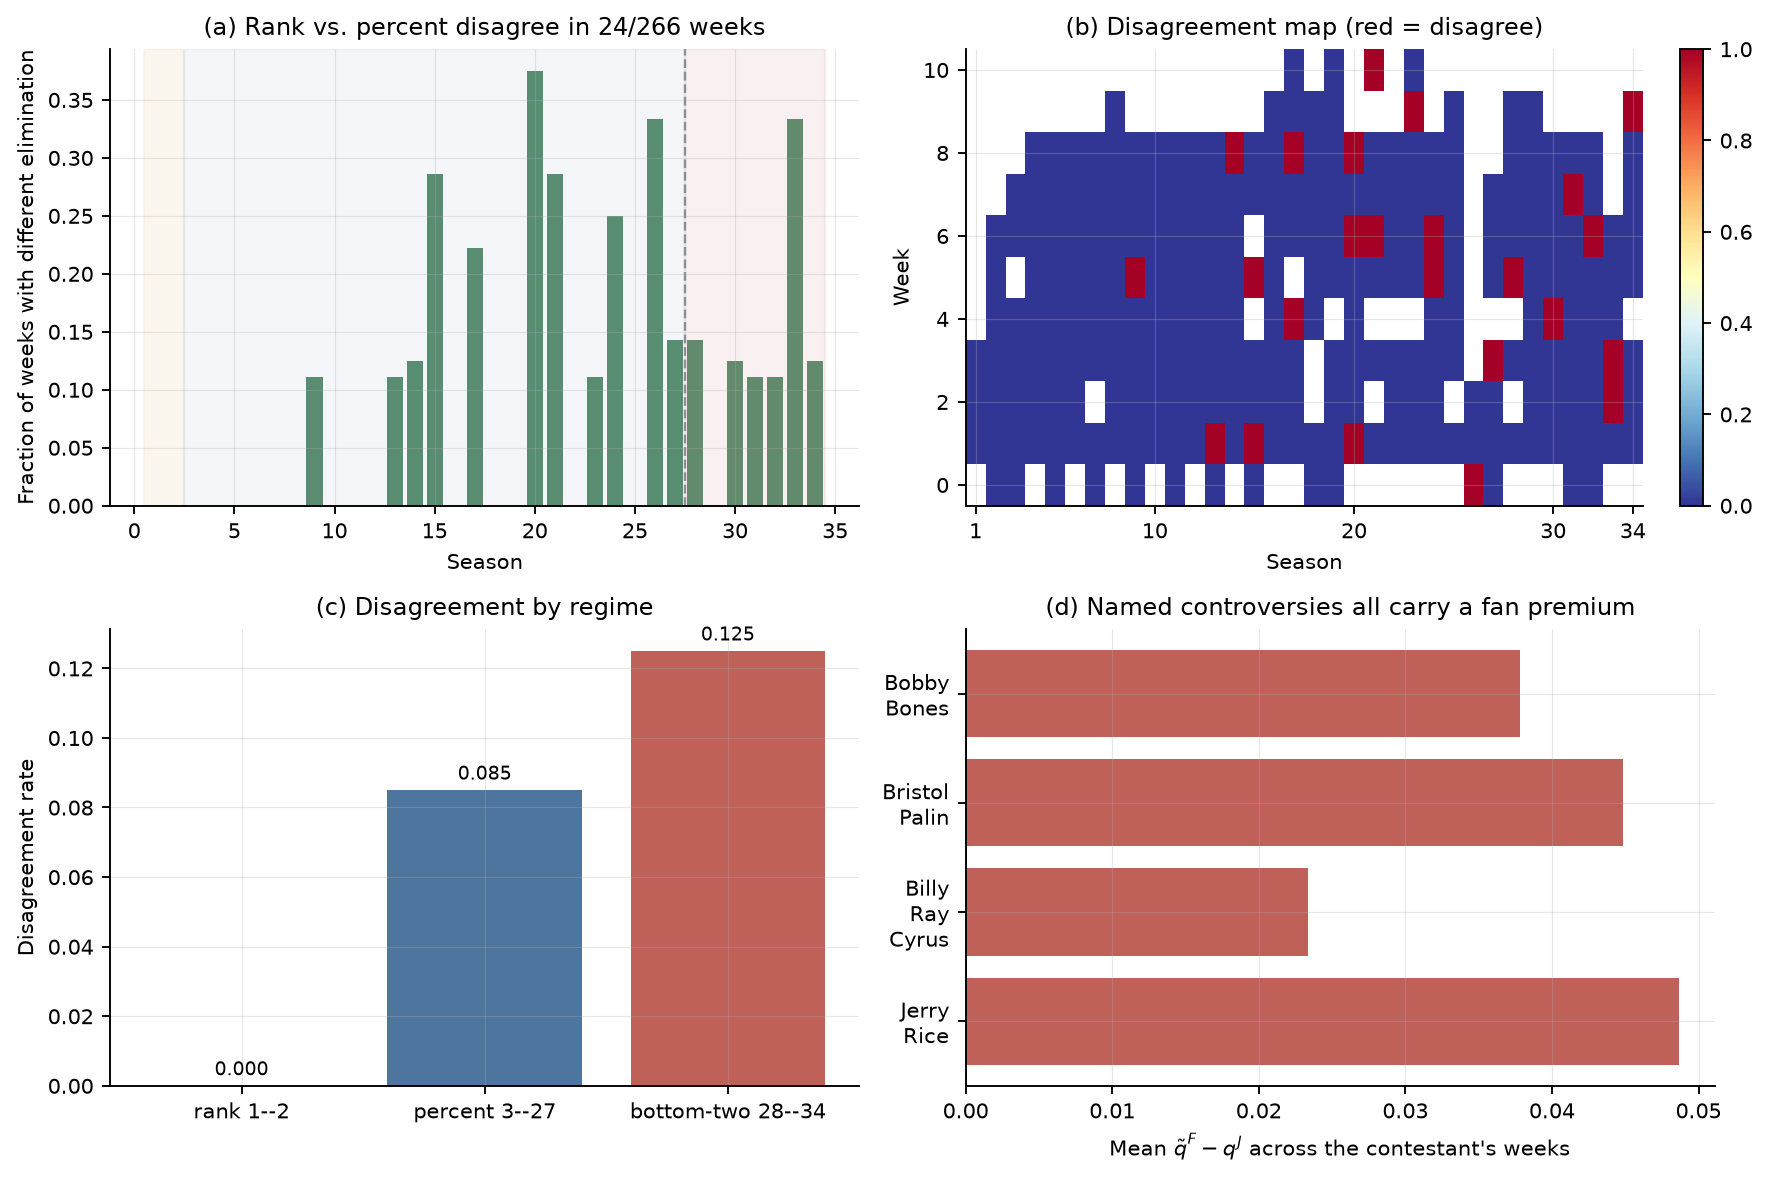
\includegraphics[width=0.94\textwidth]{figures_ext/fig09_rule_disagreement.png}
\caption{Rank versus percent rule disagreement. (a) Fraction of disagreeing eliminating weeks
by season. (b) Season-by-week disagreement map; red cells indicate that the two rules select
different couples. (c) Disagreement rate by regime. (d) Mean within-week fan premium
$\tilde q^F-q^J$ for the four named controversy contestants.}
\label{fig:disagreement}
\end{figure}

A $9\%$ disagreement rate is large in practical terms: across a typical ten-week season it
implies roughly one elimination decided by the choice of arithmetic rather than by the votes.
This is the empirical justification for treating the rule as a policy lever rather than a
presentational detail. Panel~(d) connects the statistic to the named cases --- all four
controversy contestants carry a positive mean fan premium, so they are exactly the couples
whose survival is most exposed to the rule choice.

\subsection{A Merit--Excitement Frontier for the Producers}

The evidence supports a two-dimensional view. Define a \emph{merit} objective as agreement
with the judges' ordering and an \emph{excitement} objective as the survival of couples with
strong audience support but weak judge scores. Under a judge-only rule ($w=1$) merit is maximal
but only $44.4\%$ of observed eliminations are reproduced, and the four named controversies
would end early. Under rank fusion with a heavy fan weight, those couples survive (Rice, Palin
and Bones all benefit), which raises engagement but produced the Season~27 outcome the
producers themselves reacted to. Percent fusion at $w=0.5$ sits between: it preserves judge
magnitude while leaving the audience channel enough weight to reproduce every observed
elimination in seasons 1--27.

Adding the bottom-two judge save moves the operating point further toward merit without
removing the audience channel: in $59.96\%$ of the $56$ bottom-two weeks the judges overrode
the combined-score ordering, but Figure~\ref{fig:elimevidence}(d) shows that those decisions
were typically between couples with a small combined-score gap. It is therefore a
\emph{bounded} safeguard. This is why we retain the recommendation of percent fusion with the
judge save, while noting that a producer optimising purely for close finals and audience
engagement should prefer rank fusion at a somewhat lower judge weight.

%=====================================================================
